
\documentclass{article}
\PassOptionsToPackage{latin9}{inputenc} % latin9 (ISO-8859-9) = latin1+"Euro sign"
\usepackage{inputenc}
 
 %------------------------------------------------

\usepackage{fancyvrb}

%\PassOptionsToPackage{ngerman,american}{babel}  % Change this to your language(s)
% Spanish languages need extra options in order to work with this template
%\PassOptionsToPackage{spanish,es-lcroman}{babel}
\usepackage[english]{babel}

\usepackage{listings}
\usepackage{amsmath,bm}
\usepackage{fancyhdr} % Required for custom headers
\usepackage{lastpage} % Required to determine the last page for the footer
\usepackage{extramarks} % Required for headers and footers
% \usepackage[usenames,dvipsnames]{color} % Required for custom colors
\usepackage{graphicx} % Required to insert images
% \usepackage{listings} % Required for insertion of code
\usepackage{courier} % Required for the courier font
\usepackage{lipsum} % Used for inserting dummy 'Lorem ipsum' text into the template
\usepackage{url}

%------------------------------------------------			

\PassOptionsToPackage{square,numbers}{natbib}
 \usepackage{natbib}
 
 %------------------------------------------------

\PassOptionsToPackage{fleqn}{amsmath,amssymb} % Math environments and more by the AMS 
 \usepackage{amsmath}
 
 %------------------------------------------------

\PassOptionsToPackage{T1}{fontenc} % T2A for cyrillics
\usepackage{fontenc}

%------------------------------------------------

\usepackage{xspace} % To get the spacing after macros right

%------------------------------------------------

\usepackage{mparhack} % To get marginpar right

%------------------------------------------------

\usepackage{fixltx2e} % Fixes some LaTeX stuff 

%------------------------------------------------

\PassOptionsToPackage{smaller}{acronym} % Include printonlyused in the first bracket to only show 
% acronyms used in the text
\usepackage{acronym} % nice macros for handling all acronyms in the thesis

%------------------------------------------------

%\renewcommand*{\acsfont}[1]{\textssc{#1}} % For MinionPro
% \renewcommand{\bflabel}[1]{{#1}\hfill} % Fix the list of acronyms

%------------------------------------------------

\PassOptionsToPackage{pdftex}{graphicx}
\usepackage{graphicx} 

%----------------------------------------------------------------------------------------
%	FLOATS: TABLES, FIGURES AND CAPTIONS SETUP
%----------------------------------------------------------------------------------------
\usepackage{booktabs}
\usepackage{tabularx} % Better tables
\setlength{\extrarowheight}{3pt} % Increase table row height
\newcommand{\tableheadline}[1]{\multicolumn{1}{c}{\spacedlowsmallcaps{#1}}}
\newcommand{\myfloatalign}{\centering} % To be used with each float for alignment
\usepackage{caption}
\captionsetup{format=hang,font=small}
\usepackage{subfig}  
\usepackage{color}


\definecolor{MyDarkGreen}{rgb}{0.0,0.4,0.0} % This is the color used for comments
\definecolor{Purple}{rgb}{0.75, 0.0, 1.0}
\definecolor{Blue}{rgb}{0.01, 0.28, 1.0}

\lstloadlanguages{Python} % Load Perl syntax for listings, for a list of other languages supported 
% see: ftp://ftp.tex.ac.uk/tex-archive/macros/latex/contrib/listings/listings.pdf
\lstset{language=Python, % Use Perl in this example
        frame=single, % Single frame around code
        basicstyle=\small\ttfamily, % Use small true type font
        keywordstyle=[1]\color{Blue}\bf, % Perl functions bold and blue
        keywordstyle=[2]\color{Purple}, % Perl function arguments purple
        keywordstyle=[3]\color{Blue}\underbar, % Custom functions underlined and blue
        identifierstyle=, % Nothing special about identifiers                                       
        commentstyle=\usefont{T1}{pcr}{m}{sl}\color{MyDarkGreen}\small, 
        stringstyle=\color{Purple}, % Strings are purple
        showstringspaces=false, % Don't put marks in string spaces
        tabsize=5, % 5 spaces per tab
        %
        % Put standard Perl functions not included in the default language here
        morekeywords={rand},
        %
        % Put Perl function parameters here
        morekeywords=[2]{on, off, interp},
        %
        % Put user defined functions here
        morekeywords=[3]{test},
       	%
        morecomment=[l][\color{Blue}]{...}, % Line continuation (...) like blue comment
        numbers=left, % Line numbers on left
        firstnumber=1, % Line numbers start with line 1
        numberstyle=\tiny\color{Blue}, % Line numbers are blue and small
        stepnumber=5 % Line numbers go in steps of 5
}

% Creates a new command to include a perl script, the first parameter is the filename of the script 
% (without .pl), the second parameter is the caption
\newcommand{\myscript}[2]{
\begin{itemize}
\item[]\lstinputlisting[caption=#2,label=#1]{#1.pl}
\end{itemize}
}


%----------------------------------------------------------------------------------------
%	track changes in the file
%   http://mirror.unl.edu/ctan/macros/latex/contrib/changes/changes.english.pdf
%----------------------------------------------------------------------------------------

\usepackage[deletedmarkup=xout]{changes}
%\newcommand{\todo}[1]{\textcolor{red}{{\textbf{To-Do:} #1}}}
\definecolor{darkgreen}{RGB}{0,100,0}
\definechangesauthor[name={Marten J{\"{a}}ger}, color={darkgreen}]{MJ}
\newcommand{\prnt}{\mathtt{pa}}  %% Parent(s) of term t. Direct
                                %% neighbors in graph.
\newcommand{\chld}{\mathtt{ch}} %% Child(ren) of term t. Direct
                                %% neighbors in graph.
\newcommand{\anno}{\mathtt{a}} % annotating relation, i.e., term to items

\newcommand{\pa}{\textit{pa}}  %% evtl redefine as \prnt.
\newcommand{\prob}{\ensuremath{P}}
\newcommand{\df}{\Leftrightarrow}
\newcommand{\predicate}[1]{\texttt{#1}}
\newcommand{\mathpredicate}[1]{\mathtt{#1}}
\newcommand{\argmax}{\operatornamewithlimits{arg\,max}}

 \usepackage{tikz}
\usepackage{pgffor}
\usetikzlibrary{fadings,decorations.markings,arrows,shapes,positioning}
% Margins
\topmargin=-0.45in
\evensidemargin=0in
\oddsidemargin=0in
\textwidth=6.5in
\textheight=9.0in
\headsep=0.25in

\linespread{1.1} % Line spacing

% Set up the header and footer
\pagestyle{fancy}
\lhead{\hmwkAuthorName} % Top left header
\chead{\hmwkClass\ (\hmwkClassInstructor\ \hmwkClassTime): \hmwkTitle} % Top center head
\rhead{\firstxmark} % Top right header
\lfoot{\lastxmark} % Bottom left footer
\cfoot{} % Bottom center footer
\rfoot{Page\ \thepage\ of\ \protect\pageref{LastPage}} % Bottom right footer
\renewcommand\headrulewidth{0.4pt} % Size of the header rule
\renewcommand\footrulewidth{0.4pt} % Size of the footer rule

\setlength\parindent{0pt} % Removes all indentation from paragraphs

%----------------------------------------------------------------------------------------
%	CODE INCLUSION CONFIGURATION
%----------------------------------------------------------------------------------------


%----------------------------------------------------------------------------------------
%	DOCUMENT STRUCTURE COMMANDS
%	Skip this unless you know what you're doing
%----------------------------------------------------------------------------------------

% Header and footer for when a page split occurs within a problem environment
\newcommand{\enterProblemHeader}[1]{
\nobreak\extramarks{#1}{#1 continued on next page\ldots}\nobreak
\nobreak\extramarks{#1 (continued)}{#1 continued on next page\ldots}\nobreak
}

% Header and footer for when a page split occurs between problem environments
\newcommand{\exitProblemHeader}[1]{
\nobreak\extramarks{#1 (continued)}{#1 continued on next page\ldots}\nobreak
\nobreak\extramarks{#1}{}\nobreak
}

\setcounter{secnumdepth}{0} % Removes default section numbers
\newcounter{homeworkProblemCounter} % Creates a counter to keep track of the number of problems

\newcommand{\homeworkProblemName}{}
\newenvironment{homeworkProblem}[1][Problem \arabic{homeworkProblemCounter}]{ %
\stepcounter{homeworkProblemCounter} % Increase counter for number of problems
\renewcommand{\homeworkProblemName}{#1} % Assign \homeworkProblemName the name of the problem
\section{\homeworkProblemName} % Make a section in the document with the custom problem count
\enterProblemHeader{\homeworkProblemName} % Header and footer within the environment
}{
\exitProblemHeader{\homeworkProblemName} % Header and footer after the environment
}



%%%%%%%%%%%%%%%%%%%%%%%%%%%%%%%%%%%%%%%%%%%%%%%%%%%%%%%%%%%%%%%%%%%%%%%%%
%%%%%%%%%%%%%%%%%%%%%%%%%%%%%%%%%%%%%%%%%%%%%%%%%%%%%%%%%%%%%%%%%%%%%%%%%%
%%%%%%%%%%%   SOLUTIONS %%%%%%%%%%%%%%%%%%%%%%%%%%%%%%%%%%%%%%%%%%%%%%%%%%%
%%%%%%%%%%%%%%%%%%%%%%%%%%%%%%%%%%%%%%%%%%%%%%%%%%%%%%%%%%%%%%%%%%%%%%%%%
%%%%%%%%%%%%%%   UNCOMMENT TO SHOW ANSWERS
%%%%%%%%%%%%%%%%%%%%%%%%%%%%%%%%%%%%%%%%%%%%%%%%%%%%%%%%%%%%%%%%%%%%%%%%%
%%%%%%%%%%%%%%%%%%%%%%%%%%%%%%%%%%%%%%%%%%%%%%%%%%%%%%%%%%%%%%%%%%%%%%%%%
%%%%%%%%%%%%%%%%%%%%%%%%%%%%%%%%%%%%%%%%%%%%%%%%%%%%%%%%%%%%%%%%%%%%%%%%%
\newcommand{\problemAnswer}[1]{ 
%\noindent\framebox[\columnwidth][c]{\begin{minipage}{0.98\columnwidth}#1\end{minipage}} %
}

\newcommand{\homeworkSectionName}{}
\newenvironment{homeworkSection}[1]{ % New environment for sections within homework problems, takes 
1 argument - the name of the section
\renewcommand{\homeworkSectionName}{#1} % Assign \homeworkSectionName to the name of the section 
from the environment argument
\subsection{\homeworkSectionName} % Make a subsection with the custom name of the subsection
\enterProblemHeader{\homeworkProblemName\ [\homeworkSectionName]} % Header and footer within the 
environment
}{
\enterProblemHeader{\homeworkProblemName} % Header and footer after the environment
}

%----------------------------------------------------------------------------------------
%	NAME AND CLASS SECTION
%----------------------------------------------------------------------------------------

\newcommand{\hmwkTitle}{Assignment\ \#2} % Assignment title
\newcommand{\hmwkDueDate}{Thursday,\ Oct\ 20,\ 2022} % Due date
\newcommand{\hmwkClass}{Ontology Algorithms} % Course/class
\newcommand{\hmwkClassTime}{} % Class/lecture time
\newcommand{\hmwkClassInstructor}{Peter Robinson} % 
% Teacher/lecturer
\newcommand{\hmwkAuthorName}{} % Your name

%----------------------------------------------------------------------------------------
%	TITLE PAGE
%----------------------------------------------------------------------------------------

\title{
\vspace{2in}
\textmd{\textbf{\hmwkClass:\ \hmwkTitle}}\\
\normalsize\vspace{0.1in}\small{Distributed\ on\ \hmwkDueDate}\\
\vspace{0.1in}\large{\textit{\hmwkClassInstructor\ \hmwkClassTime}}
\vspace{3in}
}

\author{\textbf{\hmwkAuthorName}}
\date{} % Insert date here if you want it to appear below your name

%----------------------------------------------------------------------------------------

\begin{document}

\maketitle

%----------------------------------------------------------------------------------------
%	PROBLEM 1
%----------------------------------------------------------------------------------------

% Chapter 1
 
\section{Information Content in Ontologies} 
\index{information content} 
 
In 1995, Resnik introduced a method for evaluating the semantic 
similarity between two concepts in an ontology with \predicate{is\_a} 
relations~\cite{Resnik1995}. Resnik's idea was to associate 
probabilities with the concepts of the ontology. Let 
$\mathcal{C}=\left\{c_1,c_2,\ldots,c_n\right\}$ be the set of concepts 
in the ontology, permitting multiple inheritance. Define a function 
$p:\mathcal{C}\longrightarrow \left[ 0,1\right]$, such that $p(c_i)$ 
is the probability of encountering an instance of class $c_i\in 
\mathcal{C}$ (Figure~\ref{fig:wordnet}).  
 
 
 
 
\begin{figure}[ht!] 
 \centering 
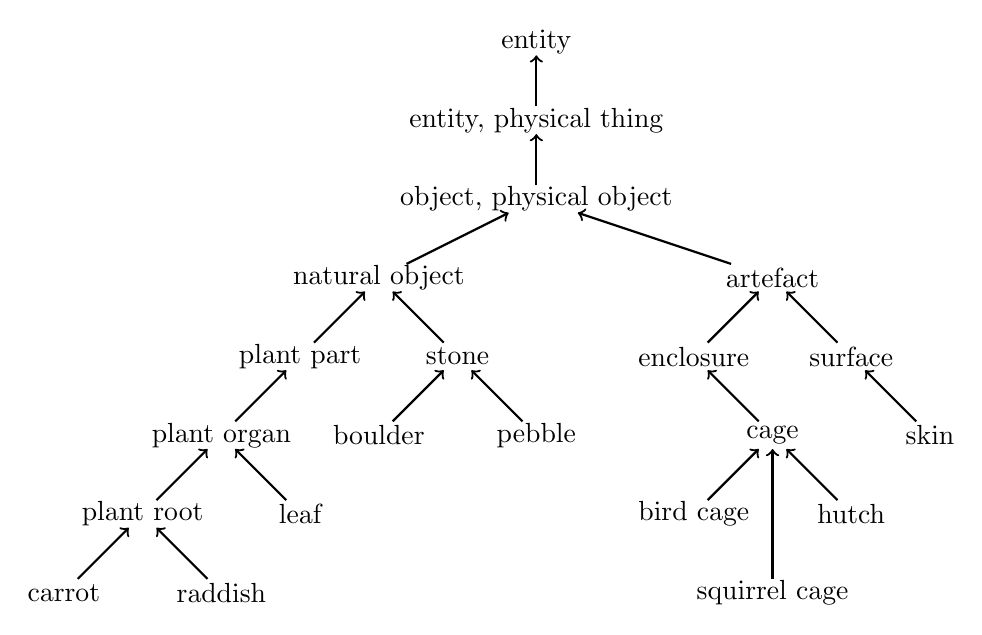
\begin{tikzpicture}
\tikzstyle{dummy} = [rectangle,minimum height=1em, inner sep=0pt, outer sep=0pt];%

\node at (5,10) [dummy] (entity) {entity};
\node at (5,9)  [dummy] (ept) {entity, physical thing};
\node at (5,8)  [dummy] (opo) {object, physical object};
\node at (8,7) [dummy] (art) {artefact};
\node at (9,6) [dummy] (surface) {surface};
\node at (7,6) [dummy] (enclosure) {enclosure};
\node at (8,5) [dummy] (cage) {cage};
\node at (7,4) [dummy] (bcage) {bird cage};
\node at (8,3) [dummy] (scage) {squirrel cage};
\node at (9,4) [dummy] (hutch) {hutch};
\node at (10,5) [dummy] (skin) {skin};
\node at (3,7) [dummy] (nobject) {natural object};
\node at (4,6) [dummy] (stone) {stone};
\node at (5,5) [dummy] (pebble) {pebble};
\node at (3,5) [dummy] (boulder) {boulder};
\node at (2,6) [dummy] (ppart) {plant part};
\node at (1,5) [dummy] (porgan) {plant organ};
\node at (0,4) [dummy] (proot) {plant root};
\node at (-1,3) [dummy] (carrot) {carrot};
\node at (1,3) [dummy] (raddish) {raddish};
\node at (2,4) [dummy] (leaf) {leaf};

\path (ept)  edge[->, thick] node[->]{} (entity) ;
\path (opo)  edge[->, thick] node[->]{} (ept) ;
\path (art)  edge[->, thick] node[->]{} (opo) ;
\path (surface)  edge[->, thick] node[->]{} (art) ;
\path (enclosure)  edge[->, thick] node[->]{} (art) ;
\path (cage)  edge[->, thick] node[->]{} (enclosure) ;
\path (bcage)  edge[->, thick] node[->]{} (cage) ;
\path (scage)  edge[->, thick] node[->]{} (cage) ;
\path (hutch)  edge[->, thick] node[->]{} (cage) ;
\path (skin)  edge[->, thick] node[->]{} (surface) ;
\path (nobject)  edge[->, thick] node[->]{} (opo) ;
\path (stone)  edge[->, thick] node[->]{} (nobject) ;
\path (pebble)  edge[->, thick] node[->]{} (stone) ;
\path (boulder)  edge[->, thick] node[->]{} (stone) ;
\path (ppart)  edge[->, thick] node[->]{} (nobject) ;
\path (porgan)  edge[->, thick] node[->]{} (ppart) ;
\path (proot)  edge[->, thick] node[->]{} (porgan) ;
\path (leaf)  edge[->, thick] node[->]{} (porgan) ;
\path (carrot)  edge[->, thick] node[->]{} (proot) ;
\path (raddish)  edge[->, thick] node[->]{} (proot) ;

\end{tikzpicture}


 \caption[Wordnet]{\textbf{WordNet}. Resnik's work defined semantic 
   similarity in \texttt{is\_a} taxonomies 
using the WordNet as an example. WordNet is a 
semantic lexicon for the English language that is used extensively by 
computational linguists and cognitive scientists. WordNet currently  
contains 155,287 English words. WordNet groups words 
into sets of synonyms called \textit{synsets} and describes semantic 
relationships between them. One such relationship is the \texttt{is\_a} 
relationship, which connects a hyponym (more specific synset) to a 
hypernym (more general synset)~\cite{Miller1995}.  
This figure shows a very small excerpt of the WordNet that 
demonstrates some of the \texttt{is\_a} 
   (subclass) relations. For instance, every \texttt{pebble} 
   is a \texttt{stone}, and every \texttt{stone} is a \texttt{natural 
     object}. Every concept in WordNet is a descendent of the root 
   term \texttt{entity}; therefore, \texttt{entity} has a probability 
   of 1, and an information content of $\log 1=0$ (i.e., whatever 
   concept we choose  
from WordNet, it has to be 
   either \texttt{entity} or a subclass of \texttt{entity}; therefore, 
   there is no added information from knowing that a random term is a 
   descendent of \texttt{entity}). On the other hand, 
   the probability of choosing a more specific term such as 
   \texttt{pebble} is much lower and the information content is 
   correspondingly higher. } 
 \label{fig:wordnet} 
\end{figure} 
 
 
Recall that $x$ 
\verb!instance_of! A and A \verb!is_a! B implies that $x$ 
\verb!instance_of! B. This means that $p$ is a monotonically 
increasing function as we move up the ontology to more general 
concepts: if $c_i$ \verb!is_a! $c_j$, then $p(c_i)\leq 
p(c_j)$. Moreover, if the ontology has a unique root node $r$, then 
$p(r)=1$. Resnik then defined the \textit{information content} of a 
concept (ontology term) as the negative log likelihood of its 
probability: 
 
\begin{equation} 
\textnormal{IC}(t)=-\log p(t). 
\label{eqn:ic} 
\end{equation} 
 
This definition makes intuitive sense. As the probability of a concept 
increases, its information content decreases (we gain  less new 
information from an observation that something common has happened 
than from an observation that something rare has happened). Moreover, 
the information content associated with the root term, which subsumes 
all concepts in the ontology and thus has a probability of 1, is zero 
because $\log 1 = 0$. Further explanations about the connections 
between this definition of information content and the definition of 
entropy in Claude Shannon's information theory are presented in 
Appendix~\ref{appendix:IC}.  
 
 
In the setting of the Gene Ontology (GO), the probability of a GO term 
$t$ is taken to be the probability that a randomly chosen protein is 
annotated to $t$, if we choose the protein from the set of all 
proteins under consideration.\footnote{Usually all proteins or all 
  annotated proteins of some organism.}  Thus, GO terms that are used 
to annotate many genes have a low information content. For instance, 
assuming that all genes are annotated to the root (the most general 
term) of the ontology, the information content of the root is 
$-\log_2(1)=0$. Intuitively, this means that if we choose a gene at 
random and discover that it is annotated to the root term of GO, this 
is not at all surprising because all genes are annotated to the 
root. On the other hand, assuming there are 256 annotated genes, the 
information content of a term used to annotate only one gene is 
$-\log_2(1/256)=8$ (recall that $2^8=256$), the information content of 
a term used to annotate two genes is $-\log_2(2/256)=7$, and so on. 
Figure~\ref{fig:ic} illustrates the relationship between information 
content and annotation frequency of ontology terms. Note that although 
Shannon's definition of entropy and information content used base 2 
logarithms, the base of the logarithm is not important for the 
analysis of semantic similarity in ontologies, logarithms to any 
base can be used for semantic similarity calculations, and in the rest 
of this chapter we will use the natural logarithm for simplicity. 
 
 
\begin{figure}[ht!] 
 \centering 
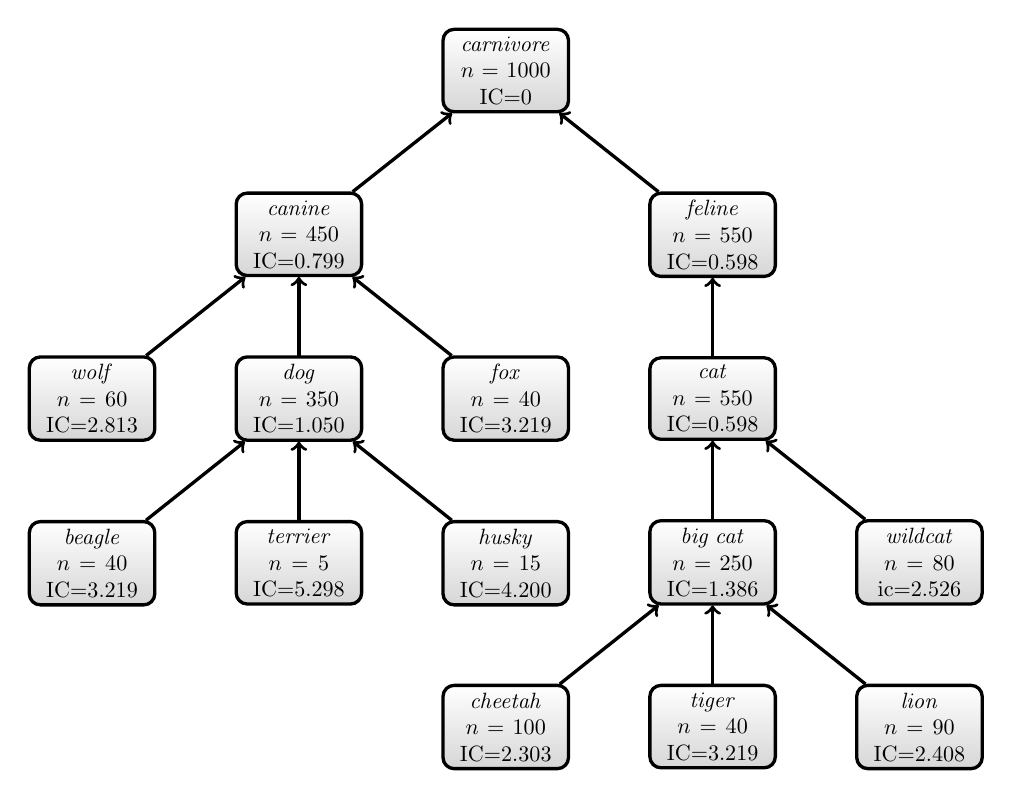
\begin{tikzpicture}
 [
 term/.style={
  rectangle,
 rounded corners, 
  minimum size=3mm,
  very thick, % border
 draw=black,
  text width=5em, 
    minimum height=2em, 
    text centered, 
  scale=0.8,
 top color=white,
 bottom color=white!60!black!40},
tip/.style={->,stealth'}]
\node (carnivore) [term] {\textit{carnivore}\\ $n=1000$\\ IC=0};
\node (canine) [term,below left=of carnivore] {\textit{canine}\\$n=450$\\IC=0.799};
\node (feline) [term, below right=of carnivore] {\textit{feline}\\$n=550$\\IC=0.598};
\node (dog) [term, below=of canine] {\textit{dog}\\$n=350$\\IC=1.050};
\node (wolf) [term, below left=of canine] {\textit{wolf}\\$n=60$\\IC=2.813 };
\node (fox) [term,below right=of canine] {\textit{fox}\\$n=40$\\IC=3.219};
\node (beagle) [term, below left=of dog] {\textit{beagle}\\$n=40$\\IC=3.219};
\node (terrier) [term,below=of dog] {\textit{terrier}\\$n=5$\\IC=5.298 };
\node (husky) [term, below right=of dog] {\textit{husky}\\$n=15$\\IC=4.200};
\node (cat) [term, below=of feline] {\textit{cat}\\$n=550$\\IC=0.598};
\node (wildcat) [term, below right=of cat] {\textit{wildcat}\\$n=80$\\ic=2.526};
\node (bigcat) [term, below=of cat] {\textit{big cat}\\$n=250$\\IC=1.386};
\node (cheetah) [term,below left=of bigcat] {\textit{cheetah}\\$n=100$\\IC=2.303};
\node (tiger) [term,below=of bigcat] {\textit{tiger}\\$n=40$\\IC=3.219};
\node (lion) [term,below right=of bigcat] {\textit{lion}\\$n=90$\\IC=2.408};
\path (canine)  edge[->,very thick] (carnivore) ;
\path (feline)  edge[->,very thick] (carnivore) ;
\path (dog)  edge[->,very thick] (canine) ;
\path (wolf)  edge[->,very thick] (canine) ;
\path (fox)  edge[->,very thick] (canine) ;
\path (cat)  edge[->,very thick] (feline) ;
\path (bigcat)  edge[->,very thick] (cat) ;
\path (wildcat)  edge[->,very thick] (cat) ;
\path (terrier)  edge[->,very thick] (dog) ;
\path (beagle)  edge[->,very thick] (dog) ;
\path (husky)  edge[->,very thick] (dog) ;
\path (lion)  edge[->,very thick] (bigcat) ;
\path (cheetah)  edge[->,very thick] (bigcat) ;
\path (tiger)  edge[->,very thick] (bigcat) ;
\end{tikzpicture}

\caption[Information Content of Ontology Terms]{\textbf{Information Content 
    of Ontology Terms}. 
 The figure shows a carnivore ontology. Imagine the ontology terms 
 have been used to annotate 1,000 documents about carnivores. If we pick 
 a document at random and learn it is annotated to the term 
 \textit{canine}, this gives us some information about the contents of 
the document, as reflected in the positive information content of 
$-\log (450/100)=0.799$. We get much more information if we learn the 
document is annotated to a more specific term such as 
\textit{terrier}, with its information content of $-\log 
(5/1000)=5.298$. 
Note that the term \texttt{dog} has 350 annotations. Assuming the 
annotations to the three child terms are disjoint, the $40+5+15=60$ 
annotations of \texttt{beagle}, \texttt{terrier}, and \texttt{husky} 
are propagated to the term \texttt{dog}, which thus must have 290 
direct annotations. On the other hand, the number of annotations of 
the term \texttt{canine} is equal to the sum of annotations of its 
children, meaning that \texttt{canine} has only propagated, but no 
direct annotations. } 
\label{fig:ic} 
\end{figure} 
 
 
\index{information content} 
\index{most informative common ancestor (MICA)} 
 
Resnik used his definition of information content to define the 
semantic similarity between two terms in an ontology. The more 
information two terms share in common, the more similar they 
are. The information shared between two terms is indicated by the 
information content of their  \emph{most 
informative common ancestor} (MICA). This is defined using the 
function $\mathtt{Anc}(t)$, which returns all of the ancestors of the 
term $t$ in the ontology, including the term $t$ 
itself.  
\label{page:definition-of-Anc} 
 
\begin{equation} 
t_{MICA(t_1,t_2)} = \argmax_{t\in \mathtt{Anc}(t_1) \cap 
  \mathtt{Anc}(t_2)}-\log p(t). 
\label{eq:mica} 
\end{equation} 
Equation~(\ref{eq:mica}) identifies the term $t$ with the maximum 
information content that is an ancestor 
of both $t_1$ and $t_2$. We 
can now define the similarity of two terms $t_1$ and $t_2$ as being 
equal to the information content of their MICA. 
 
\begin{equation} 
	\textnormal{sim}(t_1,t_2) = -\log p\left( t_{MICA(t_1,t_2)} \right) 
 = \max_{t\in 
	\mathtt{Anc}(t_1) \cap \mathtt{Anc}(t_2)} IC(t). 
\label{eq:mica-resnik} 
\end{equation} 
 
For example, the MICA of terms \textit{cheetah} and \textit{lion} in 
the ontology of Figure~\ref{fig:ic} is the term \textit{big 
  cat}. Therefore, noting that the term \textit{big cat} has the 
highest information content of any of the common ancestors of the 
terms \textit{cheetah} and \textit{lion} (Figure~\ref{fig:ic2}), we 
conclude that: 
\begin{equation*} 
\mathrm{sim}(cheetah, lion) =  \mathrm{IC}(\textit{big 
  cat}) = 1.386  
\end{equation*} 
 
 
\begin{figure}[ht!] 
 \centering 
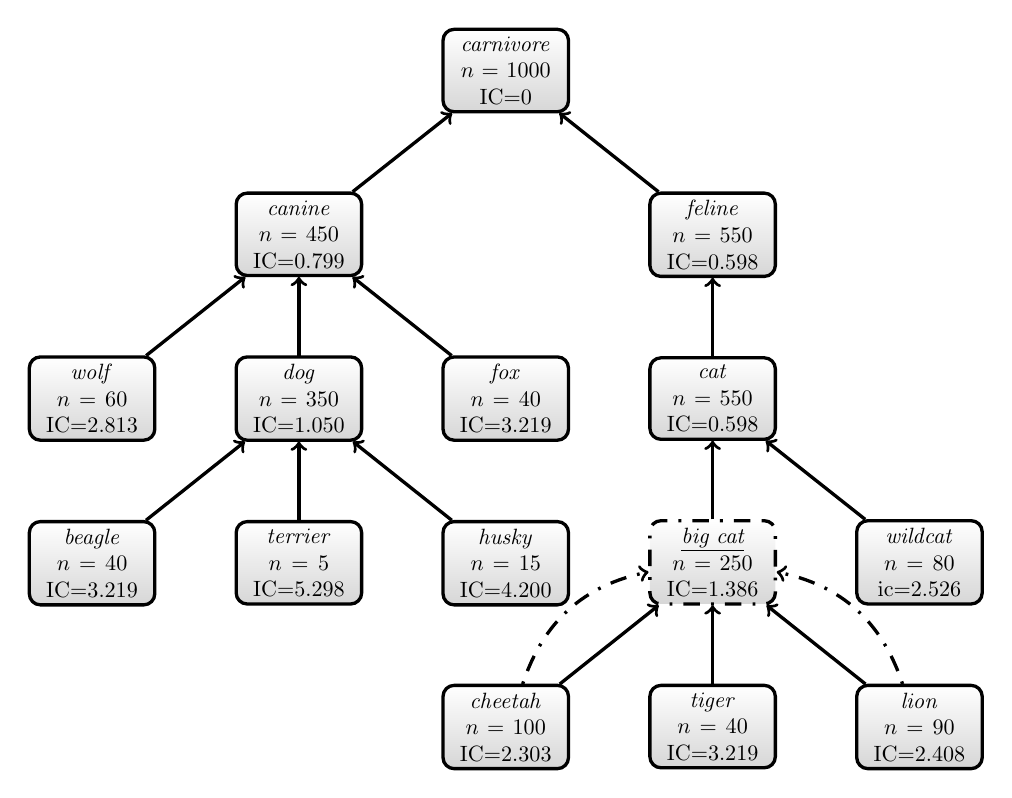
\begin{tikzpicture}
  [%
 term/.style={
  rectangle,
 rounded corners, 
  minimum size=3mm,
  very thick, % border
 draw=black,
  text width=5em, 
    minimum height=2em, 
    text centered, 
  scale=0.8,
 top color=white,
 bottom color=white!60!black!40},
 term2/.style={
  rectangle,
 rounded corners, 
  minimum size=3mm,
dash pattern=on 1pt off 4pt on 6pt off 4pt,
  very thick, % border
 draw=black,
  text width=5em, 
    minimum height=2em, 
    text centered, 
  scale=0.8,
 top color=white,
 bottom color=white!60!black!40},
tip/.style={->,stealth'}]
\node (carnivore) [term] {\emph{carnivore}\\ $n=1000$\\ IC=0};
\node (canine) [term,below left=of carnivore] {\emph{canine}\\$n=450$\\IC=0.799};
\node (feline) [term, below right=of carnivore] {\emph{feline}\\$n=550$\\IC=0.598};
\node (dog) [term, below=of canine] {\emph{dog}\\$n=350$\\IC=1.050};
\node (wolf) [term, below left=of canine] {\emph{wolf}\\$n=60$\\IC=2.813 };
\node (fox) [term,below right=of canine] {\emph{fox}\\$n=40$\\IC=3.219};
\node (beagle) [term, below left=of dog] {\emph{beagle}\\$n=40$\\IC=3.219};
\node (terrier) [term,below=of dog] {\emph{terrier}\\$n=5$\\IC=5.298 };
\node (husky) [term, below right=of dog] {\emph{husky}\\$n=15$\\IC=4.200};
\node (cat) [term, below=of feline] {\emph{cat}\\$n=550$\\IC=0.598};
\node (wildcat) [term, below right=of cat] {\emph{wildcat}\\$n=80$\\ic=2.526};
\node (bigcat) [term2, below=of cat] {\emph{\underline{big cat}}\\$n=250$\\IC=1.386};
\node (cheetah) [term,below left=of bigcat] {\emph{cheetah}\\$n=100$\\IC=2.303};
\node (tiger) [term,below=of bigcat] {\emph{tiger}\\$n=40$\\IC=3.219};
\node (lion) [term,below right=of bigcat] {\emph{lion}\\$n=90$\\IC=2.408};
\path (canine)  edge[->,very thick] (carnivore) ;
\path (feline)  edge[->,very thick] (carnivore) ;
\path (dog)  edge[->,very thick] (canine) ;
\path (wolf)  edge[->,very thick] (canine) ;
\path (fox)  edge[->,very thick] (canine) ;
\path (cat)  edge[->,very thick] (feline) ;
\path (bigcat)  edge[->,very thick] (cat) ;
\path (wildcat)  edge[->,very thick] (cat) ;
\path (terrier)  edge[->,very thick] (dog) ;
\path (beagle)  edge[->,very thick] (dog) ;
\path (husky)  edge[->,very thick] (dog) ;
\path (lion)  edge[->,very thick] (bigcat) ;
\path (cheetah)  edge[->,very thick] (bigcat) ;
\path (tiger)  edge[->,very thick] (bigcat) ;
\path (cheetah) edge[->, bend left, dash pattern=on 1pt off 4pt on 6pt off 4pt, very thick] (bigcat) 
;
\path (lion) edge[->, bend right, dash pattern=on 1pt off 4pt on 6pt off 4pt, very thick] (bigcat) ;
\end{tikzpicture}

\caption[Node-Based Semantic Similarity of Ontology Terms]{ 
\textbf{Node-Based Semantic Similarity of Ontology Terms}. 
 The semantic similarity of the terms \textit{cheetah} and \textit{lion} of 
the ontology of Figure~\ref{fig:ic} is calculated by finding their 
MICA and calculating the information content of the MICA.  } 
\label{fig:ic2} 
\end{figure} 
 
On the other hand, the MICA (and the only common ancestor) of the 
terms \textit{wildcat} and \textit{beagle} is the root of the ontology 
(Figure~\ref{fig:ic3}), meaning that they have a semantic similarity of 
zero. 
 
\begin{figure}[ht!] 
 \centering 
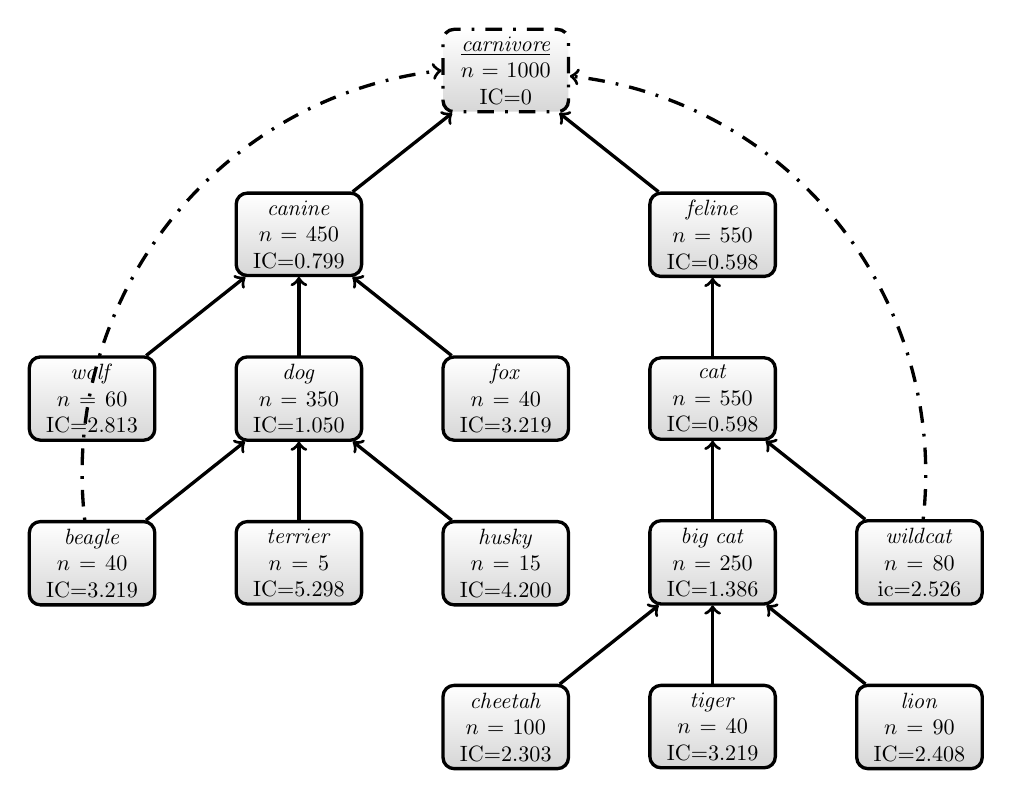
\begin{tikzpicture}
  [%
 term/.style={
  rectangle,
 rounded corners, 
  minimum size=3mm,
  very thick, % border
 draw=black,
  text width=5em, 
    minimum height=2em, 
    text centered, 
 scale=0.8,
 top color=white,
 bottom color=white!60!black!40},
 term2/.style={
  rectangle,
 rounded corners, 
  minimum size=3mm,
dash pattern=on 1pt off 4pt on 6pt off 4pt,
  very thick, % border
 draw=black,
  text width=5em, 
    minimum height=2em, 
    text centered, 
 scale=0.8,
 top color=white,
 bottom color=white!60!black!40},
tip/.style={->,stealth'}]
\node (carnivore) [term2] {\emph{\underline{carnivore}}\\ $n=1000$\\ IC=0};
\node (canine) [term,below left=of carnivore] {\emph{canine}\\$n=450$\\IC=0.799};
\node (feline) [term, below right=of carnivore] {\emph{feline}\\$n=550$\\IC=0.598};
\node (dog) [term, below=of canine] {\emph{dog}\\$n=350$\\IC=1.050};
\node (wolf) [term, below left=of canine] {\emph{wolf}\\$n=60$\\IC=2.813 };
\node (fox) [term,below right=of canine] {\emph{fox}\\$n=40$\\IC=3.219};
\node (beagle) [term, below left=of dog] {\emph{beagle}\\$n=40$\\IC=3.219};
\node (terrier) [term,below=of dog] {\emph{terrier}\\$n=5$\\IC=5.298 };
\node (husky) [term, below right=of dog] {\emph{husky}\\$n=15$\\IC=4.200};
\node (cat) [term, below=of feline] {\emph{cat}\\$n=550$\\IC=0.598};
\node (wildcat) [term, below right=of cat] {\emph{wildcat}\\$n=80$\\ic=2.526};
\node (bigcat) [term, below=of cat] {\emph{big cat}\\$n=250$\\IC=1.386};
\node (cheetah) [term,below left=of bigcat] {\emph{cheetah}\\$n=100$\\IC=2.303};
\node (tiger) [term,below=of bigcat] {\emph{tiger}\\$n=40$\\IC=3.219};
\node (lion) [term,below right=of bigcat] {\emph{lion}\\$n=90$\\IC=2.408};
\path (canine)  edge[->,very thick] (carnivore) ;
\path (feline)  edge[->,very thick] (carnivore) ;
\path (dog)  edge[->,very thick] (canine) ;
\path (wolf)  edge[->,very thick] (canine) ;
\path (fox)  edge[->,very thick] (canine) ;
\path (cat)  edge[->,very thick] (feline) ;
\path (bigcat)  edge[->,very thick] (cat) ;
\path (wildcat)  edge[->,very thick] (cat) ;
\path (terrier)  edge[->,very thick] (dog) ;
\path (beagle)  edge[->,very thick] (dog) ;
\path (husky)  edge[->,very thick] (dog) ;
\path (lion)  edge[->,very thick] (bigcat) ;
\path (cheetah)  edge[->,very thick] (bigcat) ;
\path (tiger)  edge[->,very thick] (bigcat) ;
\path (wildcat) edge[->, bend right=45, dash pattern=on 1pt off 4pt on 6pt off 4pt, very thick] 
(carnivore) ;
\path (beagle) edge[->, bend left=45, dash pattern=on 1pt off 4pt on 6pt off 4pt, very thick] 
(carnivore.west) ;
\end{tikzpicture}


 \caption[Node-Based Semantic Similarity of Ontology Terms]{ 
   \textbf{Node-Based Semantic Similarity of Ontology Terms}. The 
   semantic similarity of the terms \textit{wildcat} and 
   \textit{beagle} of the ontology of Figure~\ref{fig:ic} is 
   calculated by finding their MICA, which in this case is the root of 
   the ontology. The information content of the root of an \predicate{is\_a} 
   ontology (which annotates all items) is $-\log 1=0$.  } 
\label{fig:ic3} 
\end{figure} 
 
 
A number of modifications of Equation~(\ref{eq:mica-resnik}) have 
been developed that implicitly take characteristics of the ontology 
graph and the paths between the terms being compared into account. 
The motivation is that the measure of Resnik does not take the 
distance of the terms being compared to one another  into account, but 
only the information content of their MICA. This 
means for instance that the semantic similarity between the immediate 
children of the root term, \textit{canine} and \textit{feline} is the 
same as that of the terms \textit{beagle} and \textit{lion} according 
to Equation~(\ref{eq:mica-resnik}). As noted by Resnik, a natural way 
of estimating the similarity of two terms is merely to count the 
number of edges along the path of one node to another. In the case of 
multiple paths, the length of the shortest path is taken to be the 
distance. One problem with this is that the distance between two terms 
does not always seem to span the same semantic distance. In many 
ontologies, the semantic distance between terms (as judged by humans) 
generally gets smaller the further away one gets from the 
root. Consider for example the following two paths of length two from 
GO: (1) \textit{cornification} $\xrightarrow{part{\; }of}$ 
\textit{keratinization} $\xrightarrow{is{\; }a}$ \textit{development}, 
where \textit{cornification} is but one of myriad processes 
contributing to development; and (2) \textit{serine-type endopeptidase 
  activity} $\xrightarrow{is{\; }a}$ \textit{serine-type peptidase 
  activity} $\xrightarrow{is{\; }a}$ \textit{serine hydrolase 
  activity}, which describe serine hydrolase catalytic activities and 
seem to be much closer together in meaning. Thus, the path length by 
itself does not seem to be a good measure of semantic distance 
 
Two measures have been widely used in bioinformatics applications that 
extend Resnik's approach to take the above considerations into 
account. Lin proposed a similarity measure that is motivated by three 
intuitions about what should be considered similar in an ontology~\cite{Lin1998}: 
\begin{enumerate} 
\item sim($A,B$) is higher, the more  $A$ and $B$ have in common (the 
  commonality of two terms corresponds to their common information, 
  which is usually taken to be the information content of their MICA). 
\item sim($A,B$) is lower, the more differences exist between $A$ and 
  $B$. 
\item The maximum similarity between $A$ and $B$ is reached when $A$ 
  and $B$ are identical, no matter how much commonality they share. 
\end{enumerate} 
 
These considerations lead to a definition of similarity between two 
ontology terms $A$ and $B$ as the ratio 
between the amount of information needed to state the commonality 
between $A$ and $B$ and the information needed to fully describe $A$ 
and $B$: 
 
\begin{equation} 
\mathrm{sim}_{Lin}(t_1,t_2) = \dfrac{2\times IC(t_{MICA(t_1,t_2)})}{IC(t_1) + IC(t_2)}. 
\label{eq:semsim-lin} 
\end{equation} 
  
Since the information content of terms in 
an ontology decreases monotonically as we move up towards the root, 
$IC(t_{MICA(t_1,t_2)}) \leq \min( IC(t_1),IC(t_2))$. This implies that 
$0\leq \mathrm{sim}_{Lin} \leq 1$. In contrast, the similarity measure 
of Resnik is bounded only by the rarity of the most infrequent term 
in the ontology, say $t_s$. Then, $0\leq \mathrm{sim}_{Resnik} \leq 
-\log p(t_s)$. 
 
Intuitions 2 and 3 are reflected in the differences between 
$\mathrm{sim}_{Resnik}$ and $\mathrm{sim}_{Lin}$. Consider the 
semantic similarity between the terms \textit{beagle} and \textit{fox}. 
According to Resnik's formula, this is the information content of 
their MICA \textit{canine}, or 0.799. According to Lin's formula, this 
is weighted by the inverse of the sum of the information content of 
both terms: 
 
\begin{equation*} 
\mathrm{sim}_{Resnik}(beagle,fox) = 
IC(t_{MICA(beagle,fox)})=IC(canine)=0.799  
\end{equation*} 
\begin{equation*} 
\mathrm{sim}_{Lin}(beagle,fox) = 
\dfrac{2\times IC(canine)}{IC(beagle) + IC(fox)} = \dfrac{0.799}{3.219+3.219}=0.124 
\end{equation*} 
 
Consider now the semantic similarity between \textit{dog} and 
\textit{fox}. According to Resnik's formula, it is the same as between 
\textit{beagle} and \textit{fox} because the MICA is 
identical. For Lin's formula, on the other hand, these two terms are 
more similar, because the difference between them is less 
(Figure~\ref{fig:ic}). 
 
\begin{equation*} 
\mathrm{sim}_{Resnik}(dog,fox) = 
IC(t_{MICA(dog,fox)})=IC(canine)=0.799  
\end{equation*} 
\begin{equation*} 
\mathrm{sim}_{Lin}(dog,fox) = 
\dfrac{2\times IC(t_{MICA(dog,fox)})}{IC(dog) + IC(fox)} = \dfrac{0.799}{1.050+3.219}=0.187 
\end{equation*} 
 
 
The similarity of a term to itself is defined by its own information 
content according to  Resnik's formula, and is equal to one according 
to Lin's formula. Thus, according to Resnik's definition, the self 
similarity of a term is a function of the probability of the term, 
which is somewhat counterintuitive. For instance, 
 
 
\begin{equation*} 
\mathrm{sim}_{Resnik}(fox,fox) = IC(fox) = 3.219 
\end{equation*} 
\begin{equation*} 
\mathrm{sim}_{Lin}(fox,fox) = 
\dfrac{2\times IC(t_{MICA(fox,fox)})}{IC(fox) + IC(fox)} = \dfrac{2\times 
  IC(fox)}{2\times IC(fox)}= 1 
\end{equation*} 
 
The MICA of $(fox, fox)$ is \textit{fox}, and thus Resnik's measure 
calculates the similarity of the term \textit{fox} to itself as being 
equal to the information content of the term \textit{fox}. On the 
other hand, Lin's measure always defines the similarity of a term with 
itself to be equal to 1. 
 
Jiang and Conrath 
proposed a related distance measure~\cite{Jiang1997}. 
 
\begin{equation} 
\mathrm{dist}_{JC}(t_1,t_2) = IC(t_1) + IC(t_2) - 2\times IC(t_{MICA(t_1,t_2)}) 
\label{eq:distance-JC} 
\end{equation} 
 
If $t_1 = t_2$, then $\mathrm{dist}_{JC}(t_1,t_2) = 0$. The maximum 
distance according to this measure is between two very specific terms 
whose only common ancestor is the root. There are several ways of making a similarity measure using 
$\mathrm{dist}_{JC}$: 
\begin{equation} 
\mathrm{sim}_{JC}(t_1,t_2) = 1 - \min(1,\mathrm{dist}_{JC}(t_1,t_2)) 
\label{eq:semsim-JC} 
\end{equation} 
Another alternative transformation of the distance measure of Jiang and 
Conrath into a similarity measure defines similarity to be the inverse 
of distance, whereby 1 is added to the denominator to avoid undefined 
values, since $\mathrm{dist}_{JC}(t,t)=0$ for any term $t$~\cite{Couto2007}. 
\begin{equation} 
\mathrm{sim}_{JC}(t_1,t_2) = \dfrac{1}{1+\mathrm{dist}_{JC}(t_1,t_2)} 
\label{eq:semsim-JC2} 
\end{equation} 
 
Each of these methods (and others not mentioned here) of measuring 
semantic similarity is based upon different assumptions of what it is 
to be semantically similar in an ontology. Different measures may 
perform better for different applications.  However, as we will see below, 
Resnik's measure tends to perform well in most bioinformatics 
applications, and we will concentrate on it in the following. 
 
 


\begin{homeworkProblem}{}
  Using the carnivore ontology shown in 
Figure~\ref{fig:ic}, 
  calculate the semantic similarity of the terms \textit{husky} and 
  \textit{fox} using Equations~(\ref{eq:mica-resnik}) and 
  (\ref{eq:semsim-lin}) and the distance between them using Equation 
  (\ref{eq:distance-JC}). 
 \end{homeworkProblem}
 
 
 
\begin{homeworkProblem}{}
Using the carnivore ontology 
  shown in Figure~\ref{fig:ic}, calculate the semantic similarity of 
  the terms \textit{wild cat} and \textit{cheetah} using 
  Equation~(\ref{eq:semsim-lin}). Repeat your analysis using $\log_2$ 
  instead of the natural logarithm. What do you notice? 
 
\end{homeworkProblem}



\begin{homeworkProblem}{}
Read the following review article on Semantic similarity: \textit{Pesquita C, et al.,. Semantic similarity in biomedical ontologies. \textit{PLoS Comput Biol} (2009) \textbf{5}:e1000443.}  The authors classify semantic similarity measures according to three items:
\begin{itemize}
 \item Scope: Which entities they intend to compare, that is, GO terms versus gene products;
  \item    Data source: Which components of the ontology they use, i.e., edges versus nodes;
  \item    Metric: How they quantify and combine the information stored on those components.
\end{itemize}
Your assignment is to make a table and describe the algorithms that are explained in the article 
according to these three items.

    

    
    
\end{homeworkProblem}
\bibliographystyle{unsrt}

\bibliography{../semalgs.bib}



% %----------------------------------------------------------------------------------------
% \cleardoublepage\include{FrontBackMatter/Bibliography} % Bibliography
\end{document}